%THIS IS MERGED TO CH3
%\chapter{High Dynamic Range (HDR) Video Image Processing For Digital Glass}
%\label{hdrvideodigitalglass}
%%\section{Abstract}
%A highly parallelizable and computationally efficient
%High Dynamic Range (HDR) image compositing,
%reconstruction, and spatiotonal mapping algorithms for processing HDR video is presented in this chapter.
%The algorithms described in this chapter runs on the EyeTap Digital Glass electric seeing aid, and is designed for the use in everyday life. To validate the robustness of the algorithms, the system is tested in the extreme dynamic range situations, such as, electric arc welding. The system runs in real-time, and requires no user intervention, and no fine-tuning of parameters after a one-time calibration, even under a wide variety of very difficult lighting conditions (e.g. electric arc welding, including detailed inspection of the arc, weld puddle, and shielding gas in TIG welding), See appendix for images from a right life scenario. The approach can render video at 1920x1080 pixel resolution at interactive frame rates that vary from 24 to 60 frames per second with GPU acceleration.
%The proposed solution is implemented our system on FPGAs (Field Programmable Gate Arrays) as a proof-of-concept prototype for potentially being miniaturized and built into eyeglass frames in the future.
%
%\section{Introduction}
%%%\section{HDR seeing aids in our daily life}
%%%\subsection{Digital Glass}
%%The EyeTap Digital Eye Glass project began about 34 years ago,
%%as a seeing aid to help with specific tasks like electric arc welding,
%%as well as in general day-to-day life, by way of a general-purpose
%%computer in the form of eye glass~\cite{intelligentimageprocessing}.
%%
%%The EyeTap causes the eye itself to, in effect, function as if it were both a camera and a display.
%%Such design gives the wearer the appearance of having a glass eye
%%(See Fig.~\ref{fig:mannvis} and~\ref{fig:mannglass})
%%%Figure rightmost from Wikimedia Commons
%\begin{figure}[htb]
% %\includegraphics[width=1.0in, bb=10 10 800 800]{3_eyetaps_lowres.jpg}
% \includegraphics[width=6.0in]{ch2/diagrams/3_eyetaps_lowres.jpg}
% \caption{The MannVis WeldGlass$^{TM}$ in a welding helmet that
%          uses the EyeTap Principle for dynamic range management.
%          This stereo rig allows the wearer to see clearly in extremely high dynamic
%          range environments. }
% \label{fig:mannvis}
%\end{figure}
%%so this phenomenon has become known as the ``Glass Eye''
%%effect~\cite{mann260} 
%%(See also
%%Presence Connect, MIT Press, Teleoperators and Virtual Environments,
%%2002 August 6,
%%http://wearcam.org/presenceconnect/).
%%
%%Thus EyeTap is sometimes called the ``Glass Eye'', as well as the
%%``Eye Glass'', or simply ``Glass''.
%%Note the term ``Glass'' singular, rather than ``Glasses'' plural,
%%has been widely used to describe this invention
%%(e.g. ``EyeTap Digital Eye Glass'', figure caption,
%%Aaron Harris/Canadian Press, Monday Dec. 22, 2003).
%%
%%Example applications running on the Glass included the Visual Memory Prosthetic~\cite{mannaaai361}, and various other wayfinding aids that go beyond what is possible with optical glass.
%%
%%Some have noted the similarity of Google's Glass to our work,
%%both in its function, as well as its minimalist design,
%%(``Project Glass and the epic history of wearable computers...'',
%%By Paul Miller, The Verge, 2012 June 26, 2:42 pm).
%%See Fig.~\ref{fig:mannglass}.
%%
%%This apparatus helps the wearer see better in everyday life, while also 
%%functioning as an interface to a general-purpose wearable computer.
%%See Chapter 23 of the Encyclopedia of Interaction Design:
%%http://www.interaction-design.org
%%
%%In this paper, we present a novel application of the Digital Eye Glass
%%in dynamic range management, to help people see better in high contrast
%%scenes, and we have tested our system in the most extreme dynamic range
%%scene: TIG welding.
%
%\subsection{High Dynamic Range Imaging}
%
%Despite recent advances in camera sensing technology, state of the art digital cameras can only sense a limited dynamic range --
%much less than the human eye. This limitation is particularly pronounced when viewing an extreme dynamic range scene such when looking into oncoming automobile headlights at a license plate number on a dark road, or when doing electric arc welding.
%
%In our previous work over the last 25 years or so, 
%we overcame this limitation by combining differently exposed images of the
%same subject matter, to generate HDR (High Dynamic Range)
%images \cite{mannist}. 
%As  Robertson et al.\ state\cite{robertson2003estimation}:
%\begin{quote}
%  ``The first report of digitally combining multiple pictures of the
%  same scene to improve dynamic range appears to be
%  Mann\cite{mannist}''.
%\end{quote} 
%Over the last decade, HDR imaging has gained major interest
%and numerous solutions have been proposed to create high quality HDR
%images~\cite{mannist,comparam,robertson2003estimation,debevec2008recovering}
%and videos~\cite{kang2003high,ali2012ICASSP,irawan2005perceptually, HDRVideoCamera11}.
%However, very little focus has been put into real-time algorithms that can
%allow real-time interaction with the world.  Furthermore, the ability to run
%at interactive frame rates is particularly important for the development of
%HDR seeing aids~\cite{mann2004continuous} which can allow people to see in
%extreme dynamic range conditions, where humans would not be able to {\em see}
%with the naked eye, especially among the elderly or those with mild
%visual impairment.
%
%The key focus of this paper is to present the state-of-the-art implementation of HDR videos for extreme dynamic range condition where the scene is relatively static but high contrast. Unlike the previous approaches where images are captured with very fine bracketing (e.g., capturing 9 images which are one EV apart), we are handling a scene with bright light source and dark background, and. and captured at 60fps with 3 frames, 4 stops apart. With our setup, we have extended the dynamic range of the scene for an addition of 4 stops. 
%
%%two more examples here
%Recently, Michael et al.~\cite{HDRVideoCamera11} have proposed a system which captures HDR video with an optical arrangement having multiple sensors. One advantage of such a system is its ability to simultaneously capture differently exposed images and thus eliminates mis-registration artifacts due to motion. Alternatively, modern digital cameras such as Canon 5D Mark II can be programmed to capture videos with alternating exposures with a simple modification to the camera firmware. However, these systems record the videos on flash memory and the HDR processing (combining the differently exposed videos and tone mapping) are time-consuming offline post-processing that does not run real-time.  Therefore such a system can not be used as a real-time seeing aid, nor does the videographer receive immediate visual feedback on the recorded HDR videos. 
%
%To address these issues, a novel hardware accelerated algorithms for
%constructing HDR video from a sequence of alternating exposures, using GPUs
%(or FPGAs) for real-time HDR processing. The hardware-accelerated results
%are useful for seeing aids, as well as, being able to shoot video while
%observing the HDR video result in a viewfinder, display monitor, or other
%similar outputs. Thus, a videographer, would be able to compose the shot more
%effectively while being able to render the final result in real-time.
%
%%One contribution of this paper is the development of real-time algorithms that are parallelizable so that they can be accelerated on GPUs or other parallelizable platforms. Our HDR composition (comparametric compositing) algorithm, which is based on~\cite{ali2012ICASSP}, allows us to perform results of otherwise complex nonlinear optimizations in real-time using GPUs. Additionally, we present a dynamic range compressor that can preserve shadow and highlight detail, and is computationally efficient, thus being suitable for use for real-time video. 
%Together with our spatial-tonal mapping algorithm, which is based on a GPU
%implementation of the edge-preserving recursive filter in~\cite{GastalOliveira2011DomainTransform}, we achieved real-time (see Table~\ref{perf_table}) results that are comparable or better than some of the state-of-the-art tone mapping algorithms~\cite{reinhard2002photographic,mantiuk2006perceptual,fattal2002gradient}; especially under the extreme lighting conditions that occur, for example, in TIG welding (see Fig.~\ref{fig:welding_results}).
%
%\begin{figure}[htp]
% %\includegraphics[scale=0.2, width=3.3in, bb=0 0 800 1100, clip]{MannGlass_GoogleGlass.jpg}
% \includegraphics[width=6.0in]{ch2/diagrams/MannGlass_GoogleGlass.jpg}
% \caption{
%          Leftmost: Mann's Glass design done in collaboration with designer
%          Chris Aimone.
%          Our minimalist design of Digital Glass
%          for everyday life has an aluminium strip that runs across the
%          forehead, and is supported by two silicone nose pads attached to the
%          aluminium strip itself (i.e. no eyeglass lenses).
%          Over the right eye is the Glass (EyeTap).
%          Rightmost: Google's design (rightmost image adapted
%          from Antonio Zugaldia's image in Wikimedia Commons,
%          used under Creative Commons License).
%        }
% \label{fig:mannglass}
%\end{figure}
%
%\section{HDR Compositing}
%\begin{figure*}[t]
%\center
%\begin{subfigure}[b]{6.0in}
%\centering
%  %\includegraphics[scale=0.2, width=4.0cm, bb=0 0 800 1100]{frames/5stops/image3.jpg} 
%  %\includegraphics[scale=0.2, width=4.0cm, bb=0 0 800 1100]{frames/5stops/image2.jpg}
%  %\includegraphics[scale=0.2, width=4.0cm, bb=0 0 800 1100]{frames/5stops/image1.jpg}
%  \includegraphics[width=1.95in]{ch2/diagrams/frames/5stops/image3.jpg} 
%  \includegraphics[width=1.95in]{ch2/diagrams/frames/5stops/image2.jpg}
%  \includegraphics[width=1.95in]{ch2/diagrams/frames/5stops/image1.jpg}
%  \caption{Raw frames captured in exposure bracketing mode (-5, 0, +5 $\Delta EV$). }
%  \label{fig:image_set_multiple}
%\end{subfigure}
%
%\begin{subfigure}[b]{1.5in}
%\centering
%\includegraphics[width=1.4in]{ch2/diagrams/frames/5stops/log_5_stops.jpg}
%\caption{Log Compression}
%\label{fig:log_compress}
%\end{subfigure}
%\begin{subfigure}[b]{1.5in}
%\centering
%\includegraphics[width=1.4in]{ch2/diagrams/frames/5stops/untitled_pregamma_1_mantiuk06_contrast_mapping_0_1_saturation_factor_0_8_detail_factor_1.jpg}
%\caption{Mantiuk, R et al. \cite{mantiuk2006perceptual}}
%\label{fig:mantiuk}
%\end{subfigure}
%\begin{subfigure}[b]{1.5in}
%\centering
%\includegraphics[width=1.4in]{ch2/diagrams/frames/5stops/untitled_pregamma_1_fattal_alpha_0_25_beta_0_57_saturation_0_38_noiseredux_0_fftsolver_1.jpg}
%\caption{Fattal, R. et al. \cite{fattal2002gradient}}
%\label{fig:mouse}
%\end{subfigure}
%\begin{subfigure}[b]{1.5in}
%\centering
%\includegraphics[width=1.4in]{ch2/diagrams/frames/5stops/untitled_pregamma_1_reinhard02_key_0_07_phi_12_2_scales_range_4_lower1_upper90.jpg}
%\caption{Reinhard, E. et al. \cite{reinhard2002photographic}}
%\label{fig:mouse}
%\end{subfigure}        
%
%\begin{subfigure}[b]{6.2in}
%\centering
%  \includegraphics[width=6.0in]{ch2/diagrams/frames/5stops/final_tm_result.jpg}
%  \caption{Our result}
%  \label{fig:mouse}
%\end{subfigure}
%%        ~
%%        \begin{subfigure}[b]{0.22\textwidth}
%%                \centering
%%                \includegraphics[width=4.0cm]{frames/welding_set/dark.jpg}
%%                \caption{whatever}
%%                \label{fig:whatever}
%%        \end{subfigure} 
%\caption{Results for HDR video of extreme dynamic range.
%                 Notice that the tip of the tungsten electrode is only visible
%                 in the darkest exposure, and the background is only visible
%                 in the lightest exposure.
%                 Our result, shown in (b), is the only of the spatiotonemapping
%                 algorithms that can render the very tip of the tungsten
%                 electrode and background both clearly.
%                 (d-f) Tone mapping results from \cite{mantiuk2006perceptual,fattal2002gradient,reinhard2002photographic} using Luminance HDR program.
%                 In extreme cases, the HDR composition method by~\cite{debevec2008recovering} introduced artifacts in the shadow area, and the tone mapping algorithms further amplified these defects in the final images.
%                Our result is not only better than these tone mapping algorithms (and the only one to faithfully show the tip of the tungsten electrode)
%                but it is also capable of running in real-time.}\label{fig:welding_results}
%\end{figure*}
%
%%\begin{figure*}
%%  \center{
%%  \includegraphics[width=4.0cm]{frames/welding_set/dark.jpg}
%%  \includegraphics[width=4.0cm]{frames/welding_set/medium.jpg}
%%  \includegraphics[width=4.0cm]{frames/welding_set/bright.jpg}
%%  \includegraphics[width=4.0cm]{frames/welding_set/stage3.jpg}
%%  \includegraphics[width=4.0cm]{frames/welding_set/untitled_pregamma_1_mantiuk06_contrast_mapping_0_1_saturation_factor_0_8_detail_factor_1.jpg}
%%  \includegraphics[width=4.0cm]{frames/welding_set/untitled_pregamma_1_fattal_alpha_0_21_beta_0_82_saturation_1_noiseredux_0_05_fftsolver_1.jpg}
%%  \includegraphics[width=4.0cm]{frames/welding_set/untitled_pregamma_1_reinhard02_key_0_1_phi_1_scales_range_8_lower1_upper43.jpg}
%%  \includegraphics[width=4.0cm]{frames/welding_set/stage3.jpg}
%%  \caption{The first row shows the differently exposed images of a TIG welding scene.   a) tone mapping by \cite{mantiuk2006perceptual}}
%%  }
%%\end{figure*}
%%
%%\begin{table}[!h]
%%\resizebox{\textwidth}{8mm}{
%%\begin{tabular}{|l|r|r|p{1cm}|}
%
%%\hline
%%Tone Mapping Operator  & Time(ms) & Frames Per Second & Speed-Up using Edge-Preserved \\
%%Tone Mapping Operator  & Time(ms) & FPS & Speed-Up using Edge-Preserved \\
%%\hline
%%Mantiuk, R et al. \cite{mantiuk2006perceptual}                & 1721     & 0.58              & $143.42\times$\\
%%\hline
%%Fattal, R. et al. \cite{fattal2002gradient}                 & 1710     & 0.58              & $142.5\times$\\
%%\hline
%%Reinhard, E. et al. \cite{reinhard2002photographic}               & 154      & 6.49              & $12.83\times$\\
%%\hline
%%Edge-Preserved         & 12       & 83.33             & $1\times$\\
%%\hline
%%
%%\end{tabular}
%%}
%%\caption{This table shows the run-time of different Tone Mapping Operators and shows the speed-up of using our Tone Mapping. Our Tone
%%Mapping algorithm achieves approximately 80 frames-per-second; which is several times faster than other widely used tone mapping operators.}
%%\label{perf_table}
%%\end{table}
%%
%
%In this section, we first discuss a HDR image composition method, which is optimized for GPU or FPGA hardware implementation of electric eyeglasses \cite{mannist,robertson2003estimation,ali2012ICASSP}. Then, we present our approach in creating a real-time HDR video with our pairwise HDR composition and spatial tonal mapping method based on the edge-aware recursive filter (RF)~\cite{GastalOliveira2011DomainTransform}. Together, our proposed algorithm can run in a real-time (30fps or higher on commodity graphics hardware such as NVIDIA 460GTX at 1280x720 resolution) and requires no user intervention in the HDR creation processes.  
%
%%\subsection{Mathematical Notation}
%%We let $f$ as a function represent the \textit{camera response function} (CRF), while $f$ in a scalar context is a \textit{tonal value}, and in a matrix context $f$ is a \textit{tonal image} (e.g. a picture from a camera).  We consider a tonal value $f$ to vary linearly with pixel value but on the unit interval, and given an $n$-bit pixel value $v$ returned from a physical camera, we use $f_i = (v+0.5)/2^n$, where we have $N$ images, $i\in\{1,\ldots,N\},$ and each image has exposure $k_i$. The subscript indicates it is the $i$-th in
%%a \textit{Wyckoff set}\cite{comparam}, i.e.\ a set of images differing
%%only in exposure, and by convention $k_{i}<k_{i+1} \;\forall\; i<N$.
%%We use $f^{-1}$ as the mathematical inverse of $f$ if it has only one
%%argument, and otherwise as a joint estimator\footnote{``Joint
%%  estimator'' is used here in the sense that each photoquantity
%%  estimate depends simultaneously on multiple measurements.} of
%%photoquantity, $\hat{q}$.
%%
%\subsection{Direct Lookup method for combining exposures} \label{comp_2_lut}
%
%For the case of compositing two images with three-color (RGB) channels, one inverse comparametric lookup table (iCLUT) can be derived for each channel for a specific camera sensor. Each entry of an inverse comparametric lookup table results a joint-estimated photometric quantity, $\hat{q}$, from a pair of images captured with different exposures. Each iCLUT is composed of $256\times256$ entries of 8-bit outputs. The iCLUTs need only be calibrated once for every camera.
%
%Each entry of an iCLUT is estimated by the following equation: 
%\begin{equation}\label{joint_est}
%\begin{split}
%  \hat{q}=&f^{-1}_{\Delta EV}(f_1, f_2) \\
%  =&\frac{f^{-1}(f_1) \cdot w_1(f_1)+f^{-1}(f_2) \cdot w_2(f_2) \
%      / 2^{\Delta EV}}{w_1(f_1)+w_2(f_2)}\\
%%\end{cases}
%\end{split}
%\end{equation} 
%where $f_1$ and $f_2$ are the pixel values from a pair images under different exposure settings; $\Delta EV$ is the exposure difference between $f_1$ and $f_2$; $f^{-1}$ is the inverse camera response and $w$ is the certainty function, proposed by Mann\cite{mannist}
%%The camera response function (CRF) f can be determined using the method described by Manders and Mann \cite{mannist}.
%%To construct this look-up-table, we first estimate the response function of the camera along with its certainty function \cite{mannist}.
%%An estimate, $\hat{q}$, of the photoquantity is computed from the pixel (tonal) values $f_1$ and $f_2$. 
%%This can be estimated by the weighted average of the $f_1$ and $f_2$ with respect to their certainty functions $w_i$ and the response function $f$ of the camera.
%
%%\begin{algorithm}
%%\begin{algorithmic}
%%\Procedure{RF}{$I$}
%%	\State $\left[\frac{dH}{dx}, \frac{dH}{dy}\right] \gets Calculate\_Gradient(I)$
%%	\State $Transpose\_Image(I)$ \Comment{Rows become columns}
%%	\State $RF\_Y\left(I, \frac{dH}{dx}\right)$            \Comment{To process the rows}
%%	\State $Transpose\_Image(I)$ \Comment{Revert to original image}
%%	\State $RF\_Y\left(I, \frac{dH}{dy}\right)$            \Comment{To process the columns}
%%\EndProcedure
%%\end{algorithmic}
%%\caption{Computation of a single entry in an iCLUT}
%%\label{RF_pseudo}
%%\end{algorithm}
%
%
%%
%%However, in extreme cases the images are several stops apart. It is important that the certainty function provides additional weighting to the brighter image to reduce the gain $2^{\Delta EV}$ to the shadow area in the last step.
%
%\subsection{HDR Composition for 3 or more Images} \label{comp3_set} 
%For the case of constructing HDR images from N images (for N $\ge$ 3), we compute $log(N)$ levels of pairwise estimate of the photometric quantities, $\hat{q}_{h,i}$, read as the $ith$ pairwise estimate of photometric quantity at level $h$. At the top level, we compute $\hat{q}_{log(N),i}$ using iCLUT generated by Eq.~\ref{joint_est}. For each of proceeding level, its corresponding set of $\hat{q}_{h,i}$ is estimated by: 
%\begin{equation}
%\hat{q}_{h,i}=\frac{\hat{q}_{h-1,j}\hat{w}_{h-1,j}+\hat{q}_{h-1,j+1}\hat{w}_{h-1,j+1}/ 2^{\Delta EV}}{\hat{w}_{h-1,j}+\hat{w}_{h-1,j+1}}
%\end{equation}
%where
%\begin{equation}
%\hat{w}_{h,i}=\max(\hat{w}_{h-1,j},\hat{w}_{h-1,j+1})
%\end{equation}
%
%
%%\begin{equation}
%%\hat{q_i}=f^{-1}_{\Delta EV}(f_i, f_{i+1}), i \in \{1,..,N\}
%%\end{equation}
%
%%Then, we combine the individual photoquantity $\hat{q_i}$ with the
%%certainty values $\hat{w_i}$ computed from last step with:
%%\begin{equation}
%%\hat{q}=g(\hat{q_i}, \hat{q}_{i+1}, ... , \hat{q}_{N-1}, \hat{w_i}, \hat{w_{i+1}},...,\hat{w_{N-1}})
%%\end{equation}
%%to create our final estimate of $\hat{q}$.  For the case of 3 images,
%%the function $g$ can be implemented as a simple weighted average of
%%the $q_1$ and $q_2$ with respect to the certainty values $\hat{w_1}$ and
%%$\hat{w_2}$:
%%\vspace{-.1in}
%%\begin{equation}
%%\begin{split}
%%  \hat{q} = g(\hat{q}_1, \hat{q}_2, \hat{w}_1, \hat{w}_2) = \frac{\hat{q}_1 \cdot
%%    \hat{w}_1 + \hat{q}_2 \cdot \hat{w}_2 / 2^{\Delta EV}}{\hat{w}_1+\hat{w}_2}
%%\end{split}
%%\end{equation}
%
%
%%One advantage of our proposed algorithm is that we have reduced the problem
%%into sub-steps that we can easily optimize for specific algorithm, and
%%can provide a significant speedup in those cases. 
%%\begin{figure}
%%  \includegraphics[width=3.5in]{siggraph2010_ch2/diagrams/4_composite_2.pdf}
%%  \caption{Composition of HDR images using our pairwise approach for
%%    combining four LDR images, $f_1$, $f_2$, $f_3$, and $f_4$. The final
%%    estimate of the photoquantity $\hat{q}$ then undergoes our hardware-accelerated tonemapping algorithm.  }
%%  \label{composite3}
%%\end{figure}
%
%By capturing 4 images with $\Delta EV=4$, the dynamic range of the HDR image spans a total of 20 stops $(2^{20}=1,048,576)$ approximately a million to one contrast ratio. To display such wide range on the LDR display, the photoquantity $\hat{q}$ will be compressed with a multi-scale spatial-tonal mapping algorithm.
%%
%% history here
%%
%
%\subsection{Global Histogram Equalization}
%With the power/logarithmic compression, the $\hat{q_c}$ often cluster in a narrow range of values and thus under-utilizing the displayable range (see Fig.~\ref{fig:welding_results} (c)). To re-distribute $\hat{q_c}$ to have a uniform occupancy across the possible displayable range, we adopted the histogram equalization (HE) as the technique to recover the global contrast from the HDR image. Since $\hat{q_c}\epsilon[0,max(\hat{q_c}))$, normalization is required to bound $\hat{q_c}$ in a known range. To perform HE, we need to construct a histogram of the image as well as the cumulative sum of the histogram:
%%h($\cdot$) as equalization operator and $\hat{q_h}$ as equalized estimator,
%\begin{equation} \label{histogram_regular}
% \hat{q_h}=HE(\hat{q_c})=\frac{cs(\hat{q_c})-cs_{min}}{M-cs_{min}}max(\hat{q_c})\\
%\end{equation}
%where $M$ denotes the number of pixels in the image and $cs(v)$ results the cumulative sum of $v$ from its histogram. It is known that Equation~\ref{histogram_regular} may over-stretch $\hat{q_c}$ at spikes in a histogram (e.g. $h_k \gg h_{k+1}$ and $h_k \gg h_{k-1}$). This may yield undesirable result since $\hat{q_c}$ is concentrated in a narrow range of values. The outcome of the equalized image then compresses the contrast of brightest and darkest light values and results a LDR like image. To resolve this behaviour, we apply histogram modification proposed by~\cite{lee2012power}:
%\begin{equation} \label{histogram_regular}
% m_k=\frac{\log(h_kh_{max}10^{-\mu}+1)}{\log(h_{max}^{2}10^{-\mu}+1)}\\ 
%\end{equation}
%\begin{equation}
% cs(k)=\displaystyle\sum\limits_{i=0}^{k-1}m_k
%\end{equation}
%where $m_k$ is the modified value of the original value of histogram at bin k, $h_k$. The choice of $\mu$ moderates the change to the histogram. For large $\mu$, the histogram becomes nearly uniform, whereas, for small $\mu$ $\ll$ 1, the histogram remains approximately unchanged. We have chosen $\mu$ = 5 which results a much more uniformly distributed histogram. Consequently, it reduces the over-stretching effect of equalization.
%
%\section{Multi-scale Spatial Tonal Mapping}
%%halo free, much less artifact than the other two (compare with fatal,etc...)
%%With a global tonal mapping operator, the HDR result obtained from the previous section appears relatively low in contrast and saturation when dealing with extreme dynamic range scene (See Figure~\ref{lamp_set}). To improve the visual appearance of the images on LDR display, we can compress the HDR image based on the not only tonal information, but also spatial information such as gradient and edges. Although a number of tone mapping algorithms had been proposed, very few tone mapping algorithm been designed for the real-time video usage. Particularly, the tone mapping which shows high quality results often involves non-linear optimizers which has a high complexity and difficult to be parallelized due to its non-deterministic runtime. On the other hands, results from \cite{reinhard2002photographic}, which has low computation requirements and easy to parallelized, produce poor looking results with halo artifacts, low contrast, and non-natural looking results. Moreover, some of the tone mapping operators are only designed for images and produce temporal artifacts such as flickering and color shifting throughout the process.
%%Recently, a computationally efficient edge-preserving filter \cite{chen2007real, GastalOliveira2011DomainTransform} has shown promising results in performing tone mapping on HDR images. %The recursive filter (RF) ~\cite{GastalOliveira2011DomainTransform} is shown to be particularly well-suited for decomposing the image in real-time on graphics hardware.
%Our approach for real-time tone mapping and composition, which is based on \cite{GastalOliveira2011DomainTransform} and \cite{farbman2008edge}, provides the natural looking and stable results among a large variety set of conditions (see Fig.~\ref{fig:welding_results} for comparison).
%%The contribution of our work is the design of a complete HDR algorithm that can run on graphics hardware or FPGAs in the future.
%%list a few tone mapping algorithms here%
%%see figure for the L value.
%%see the compressed value
%%decomposition
%%detail layers
%%controls
%%
%%see the final value
%%\subsection{Global Dynamic Range Compressor}
%To compress the high dynamic range images we first estimate the log luminance, $L_c$, of the image based on the final estimate of photoquantities on the RGB channels, $\hat{q}_r$, $\hat{q}_g$, $\hat{q}_b$, from section 2.2.
%\begin{equation}
%L_c = log(0.2989*\hat{q_r} + 0.5870*\hat{q_g} + 0.1140*\hat{q_b} + 1).
%\end{equation}
%Then, the dynamic range of the luminance channel is compressed using a logarithmic compressor with a simple offset to avoid negatives values.
%\begin{equation}
%L_c = log(L+1).
%\end{equation}
%Alternatively, we found that we can achieve a more natural looking, but less contrast result with the following compressor.
%\begin{equation}\label{lum_equation_2}
%L_c = L^{l/\gamma}
%\end{equation} where $\gamma \ge 1$ and $c$>0.
%
%Then, the $L_c$ is normalized and compressed to the range $[0,1]$. Then, we can adjust the range, which has later effect on the detail extraction, with the $s$ and $d$ parameters (typically set to $s=8.0$, $d=5$).
%\begin{equation}\label{lum_equation_3}
%L = s*L_c+d
%\end{equation}
%In our setup, we have applied a moving average filter on $max_L$ and $min_L$ to avoid flickering due to any sudden luminance changes in the scene.
%
%\subsection{Local Contrast Enhancement}
%The global tone mapping, such as logarithmic compression, from the last step provides us a base image which is often lacking contrast. We can enhance the local contrast (spatial-tonal mapping) with the multi-scale edge-preserving decomposition method. This method is found to be effective for compressing HDR images at extreme cases (see the clear rendition of the tip of the tungsten electrode with our proposed method in Fig. 1b).
%To extract details from the image and enhance their local contrast, we first create the multi-scale edge-preserved smoothed image $J_i$ where i $\in\{1,..,M\}$ using the recursive filter (RF) discussed in \cite{GastalOliveira2011DomainTransform}.
%\begin{equation}\label{lum_equation_4}
%J_i = RC (L, \sigma_s, \sigma_r, k)
%\end{equation}
%where $\sigma_s$ and $\sigma_r$ are the filter spatial and range standard deviation, and k is the number of iterations the filter smooths the image. In particular, we use $\sigma_s$ = 20, $\sigma_r$ = 0.0825 for $J_1$; $\sigma_s$ = 50, $\sigma_r$ = 0.165 for $J_2$; $\sigma_s$ = 100, $\sigma_r$ = 0.335 for $J_3$ and $k=1$. We obtain the detail layers $D_i$ by finding the difference between $J_{i-1}$ and $J_i$, with $J_0=L$, where each succession of the detail layer contains coarser details than the previous layer. The detail layers are weighted and summed to reduce to a single contrast mask $L_f$ as the following:
%\begin{equation}
%L_f = 0.9*J_M + \sum_{i=0}^{M-1}{a_i D_i}
%\end{equation} where $a_i$ is the desired weight for each layer. In our setup, we have used $a_0=0.4$, $a_1=0.3$, $a_2=0.3$ which emphasize the texture from the layer containing the finest details. By our observation, this setting allows greater local contrast of tonal values at the extreme bright and dark areas of the scene. To obtain a displayable output image, we compress the photoquantity $\hat{q}$ using the contrast mask in eq.\ref{lum_equation_4} and quantize the results to the standard 24 bit RGB pixel values:
%\begin{equation}
%\begin{split}
%f &= round(255.0*(\hat{q}/10^{L})^{\gamma} \cdot L_f), \\
%\end{split}
%\end{equation}
%
%
%Table~\ref{table:layers}.
%\vspace{-0.5cm}
%\begin{table}[!h]
%\center
%\caption{The parameters for the 3 detail layers used in our system.}\label{table:layers}
%\begin{tabular}{|c|c|c|c|}
%\hline
% & $J_1$ & $J_2$ & $J_3$ \\
%\hline
%$\sigma_s$ & 20.0 & 50.0 & 100.0 \\
%\hline
%$\sigma_r$ & 0.0825 & 0.165 & 0.335 \\
%\hline
%\end{tabular}
%\end{table}
%From our experiment, this filter is more computationally efficient than bilateral filter n large kernel size. This is a critical requirement to our HDR compression algorithm as the runtime remains constant regardless of the parameters settings. Furthermore, does not introduce temporal artifacts (such as flickering) and the results is consistent (e.g., the histogram equalization approach often result in inconsistent results under difficult lighting condition). This is critical in HDR video because any incoherence between the adjacent frames can be distracting to the audience.
%Once we have obtained the smoothed edge-preserving images, the detail layers from is extracted by subtracting the adjacent images from the stack.
%\begin{equation}
%D_i = J_i - J_{i+1}
%\end{equation} where $J_0=L$, and i $\in \{0,..,K-1\}$.
%Then, we can compose our results by first normalizing the $J_N$ channel as our base image with the following linear mapping:
%\begin{equation}
%B = \frac{J_K - min_J}{max_J - min_J}
%\end{equation}
%where $[min_J, max_J]$ is the desired range we would like for the LDR image.
%where $max_J$ and $min_J$ are the desire range we would like to mapped to our LDR.
%where the parameter $\gamma$ controls the saturation in the final image, and we typically set them between $0.5$ to $0.7$.
%
%
%Overall, there are two main advantages of using the edge-preserving filter proposed by \cite{GastalOliveira2011DomainTransform}. First, the parameters $\sigma_s$ and $\sigma_r$ empower users to refine their emphasis of detail enhancements. Second, the fine tuning of $\sigma$ parameters helps minimizing the halo artifacts when comparing to traditional image decomposition based on laplacian pyramid. Qualitatively, the output of our HDR rendition is comparable to many other approaches as shown in Fig~\ref{fig:welding_results}.
%%It is worth noting that this tone mapping algorithm is size dependent. For higher resolution videos, it may be necessary to use additional layers (e.g., 4 layers instead of 3 in this case). Fortunately, the algorithm proposed is independent of other parameter settings such as brightness, contrast, and detail manipulation, since the size of the video is constant. These properties are critical to the design of a HDR system that would be used in day-to-day life. Furthermore, our proposes solution shall be scalable to higher resolution as more capable hardware becomes available in the future.
%\section{Performance}
%%The algorithms described in previous sections were specifically chosen and designed to be parallelized on GPUs and simplified for direct hardware implementation on FPGAs.
%%To show the feasibility of our approach, the Direct LUT method described in Section~\ref{comp_2_lut} were implemented with the 3 alternating frames on FPGAs.
%\subsection{GPU}
%\begin{table}[!h]
%\center
%\begin{tabular}{|l|r|r|}
%\hline
%%Tone Mapping Operator  & Time(ms) & Frames Per Second & Speed-up \\
%\bf{Tone Mapping Operator} & \bf{FPS} & \bf{Speed-up}\\
%\hline
%Mantiuk, R. et al. \cite{mantiuk2006perceptual}     & 0.58              & $143.42\times$\\
%\hline
%Fattal, R. et al. \cite{fattal2002gradient}        & 0.58              & $142.5\times$\\
%\hline
%Reinhard, E. et al. \cite{reinhard2002photographic}     & 6.49              & $12.83\times$\\
%\hline
%Implemented Edge-Preserving Method          & 83.33             & $1\times$\\
%\hline
%\end{tabular}
%\caption{This table shows the run-time of different Tone Mapping Operators and the speed-up of using our implemented method. Our implementation 
%achieves approximately 80 frames-per-second; which is several times faster than other tone mapping operators.}
%\label{perf_table}
%\end{table}
%
%Computation using GPU maximizes acceleration on algorithms that run on a large matrix with independent element operations. Our proposed HDR algorithm heavily relies on per pixel operation without much cross dependencies with neighbour pixels. In the following discussion, we layout the runtime cost of each operation in milliseconds, benchmarked on a NVIDIA 460GTX, over 150 videos at the resolution of 1280x720. The operations of pixel-to-photoquantity conversion and the compression by logarithm consume on average of $1.5ms$. Normalization on images are done using efficient min/max finder from NVIDIA's CUBLAS library, which costs around $0.8ms$ per call. The spatial tone mapping is the least parallelizable part of the process, which consumes up to $12ms$. The edge-preserving filtering for three layers executed in parallel takes up $11ms$ of runtime, becomes the main contributor to the overall latency in our proposed HDR pipeline. This is due under utilization of available thread pool of the GPU architecture. Per iteration the RF only requires as many threads as the size of one dimension of the image multiplied by the number of color channels. In our proposed implementation, we launch the filter on a monotone channel, $L$, to reduce the total amount of computation required. Other optimization technique such as matrix transpose is applied to ensure coalesced memory access patterns. The remainder of $1ms$ runtime is contributed by the contrast enhancement stage after obtaining the layers using RF. Overall, the HDR composition and tonal range compression algorithm cost $17ms$ (~60fps) on average, and that is suitable for real-time system. 
%%The general rule in GPU computing is to avoid excessive memory transfer between the machine and graphics card. In our application, since every step can be computed using GPU, the memory transfer is only required upon receiving a new frame. Since the transfer overhead with latency is as low as 1$ms$ per frame per direction (e.g., host to device or device to host), it is relatively insignificant comparing to the latency due to the construction of HDR image. Global memory access on GPU is usually expensive in comparison to shared memory and thread cache. Frequent access to read/write global memories as intermediate update could cause high latency and drop performance of the construction. Another expensive operation is due to thread synchronization after each kernel call. Therefore, 
%
%%\begin{table}[!h]
%%\center
%%\caption{Average latency per stage of HDR construction for a $1280\times720$ image on a NVIDIA Tesla C2050 with 3 detail layers.}
%%\begin{tabular}{|l|c|}
%%\hline
%%Operation & Time (ms) \\
%%\hline
%%Light space conversion & 1.5 \\
%%\hline
%%Local Contrast Enhancement with RF & 24.0 \\
%%\hline
%%\end{tabular}
%%\end{table}
%
%
%%\subsection{FPGA}
%%
%%The algorithm which uses direct look up table is implemented on a Spartan-6 LX45 FPGA device for its low power consumption and portability. %(See Fig~\ref{fig:FPGAHDRchitecture}). 
%%The supply power measured for the system is 1.448W, thus it allows the application to run for around $20$ hours on a typical rechargeable battery with capacity of $5800$mAh.
%%The board contains High Definition Multimedia Interface (HDMI) input ports used to receive video in $720\times480$ at 60 frames per second, and output HDMI ports used to transmit HDR video frames. 
%%Two differently exposed video frames of the same subject matter are supplied via the HDMI input in rapid succession, in an alternating order.
%%The frames are stored into memory and read out concurrently for composition.
%%The 128MB of DDR SDRM (Micron MT47H64M16-25E, 16-bit data width) on the board is configured to run at 625MHz data rate to store video frames.
%%The board also contains 2.1Mbits (116x18432bits) Block RAM (BRAM) in total, which are used for line buffers and to store pre-computed LUT results.
%%
%%The post processing starts by compressing the produced HDR images with a square root.
%%Then it converts the color space from RGB to YCrCb, in order to save the resources that needed for implementation. Converted luma channel is convolved with multi-stage a 5-by-5 Gaussian Kernel for extracting two layers of edges from the original HDR image.
%%The edges are then scaled and added back to the original image for bringing back the detailed textures.
%%
%%The 4-up display mode was created to provide a real-time visualization of multiple exposures,  
%%  enabling the user to simply point a camera and see the frames that comprise the HDR composition. 
%%This allows for easier testing and calibration of the input frames for HDR video processing %(See Fig~\ref{diagram_4up}).
%%The maximum latency of the implemented logic is 223ns, whereas the DDR2 memory access used up 80 percent of the processing time.
%
%%\begin{figure}
%%\center
%% \includegraphics[width=7.5cm]{fpga_images/acmmm12_fpga.pdf}
%% \caption{FPGA-based HDR architecture for the 4-up display capabilities.}
%% \label{fig:FPGAHDRchitecture}
%%\end{figure}
%
%%\subsubsection{Real-time HDR Streaming Using 2 frames}
%%Real-time HDR composition of 2 differently exposed frames was implemented using direct look-up tables (LUTs).
%%For combining two images~\cite{ccece2012hdrEyetap}, pre-computed 8-bit values are stored into Block RAMs (BRAM).
%%In order to implement one LUT, it requires 65556-entries (256 x 256) times 8 bits per entry, which is equivalent of 524kbits. 
%%This requires 1.5Mbit (524kbits x 3 channels of RGB) to cover the two images with 8-bit RGB color space.
%%Since the Spartain-6 FPGA contains 2.1Mbits of BRAM, a more efficient memory utilization method is required to enable HDR involving more than two frames. 
%
%%\subsubsection{4-up HDR display, enabled by FPGA}
%%Push buttons and switches connected to the FPGA are configured such as to enable switching the order of dark, medium, bright frames, and turning on/off 4-up mode. 
%%To be included as a hand-held screen for the final prototype for portable real-time HDR device, this 4-up screen enables users to calibrate exposures quickly and accurately on the go.  
%
%%In the process of implementing the 4-up display, a constraint was put on the design to ensure that no change was required to the original data path. 
%%This requirement was crucial to the overall modular design of our FPGA HDR architecture. 
%%This only adds two modifications to the original data path, both of which are controlled via push-button switches. The switches allow for easy change to the original data path without the 4-up - useful for when the full-screen or eyeglass-mounted display or EyeTap resolution is desired for just the combined HDR video.
%
%%diagrams for the flow
%%fixed aperture (DOF) 
%%low ISO (noise)
%%only alter the shutter speed
%
%\section{Results and Applications}
%
%\begin{figure}
%\center
% 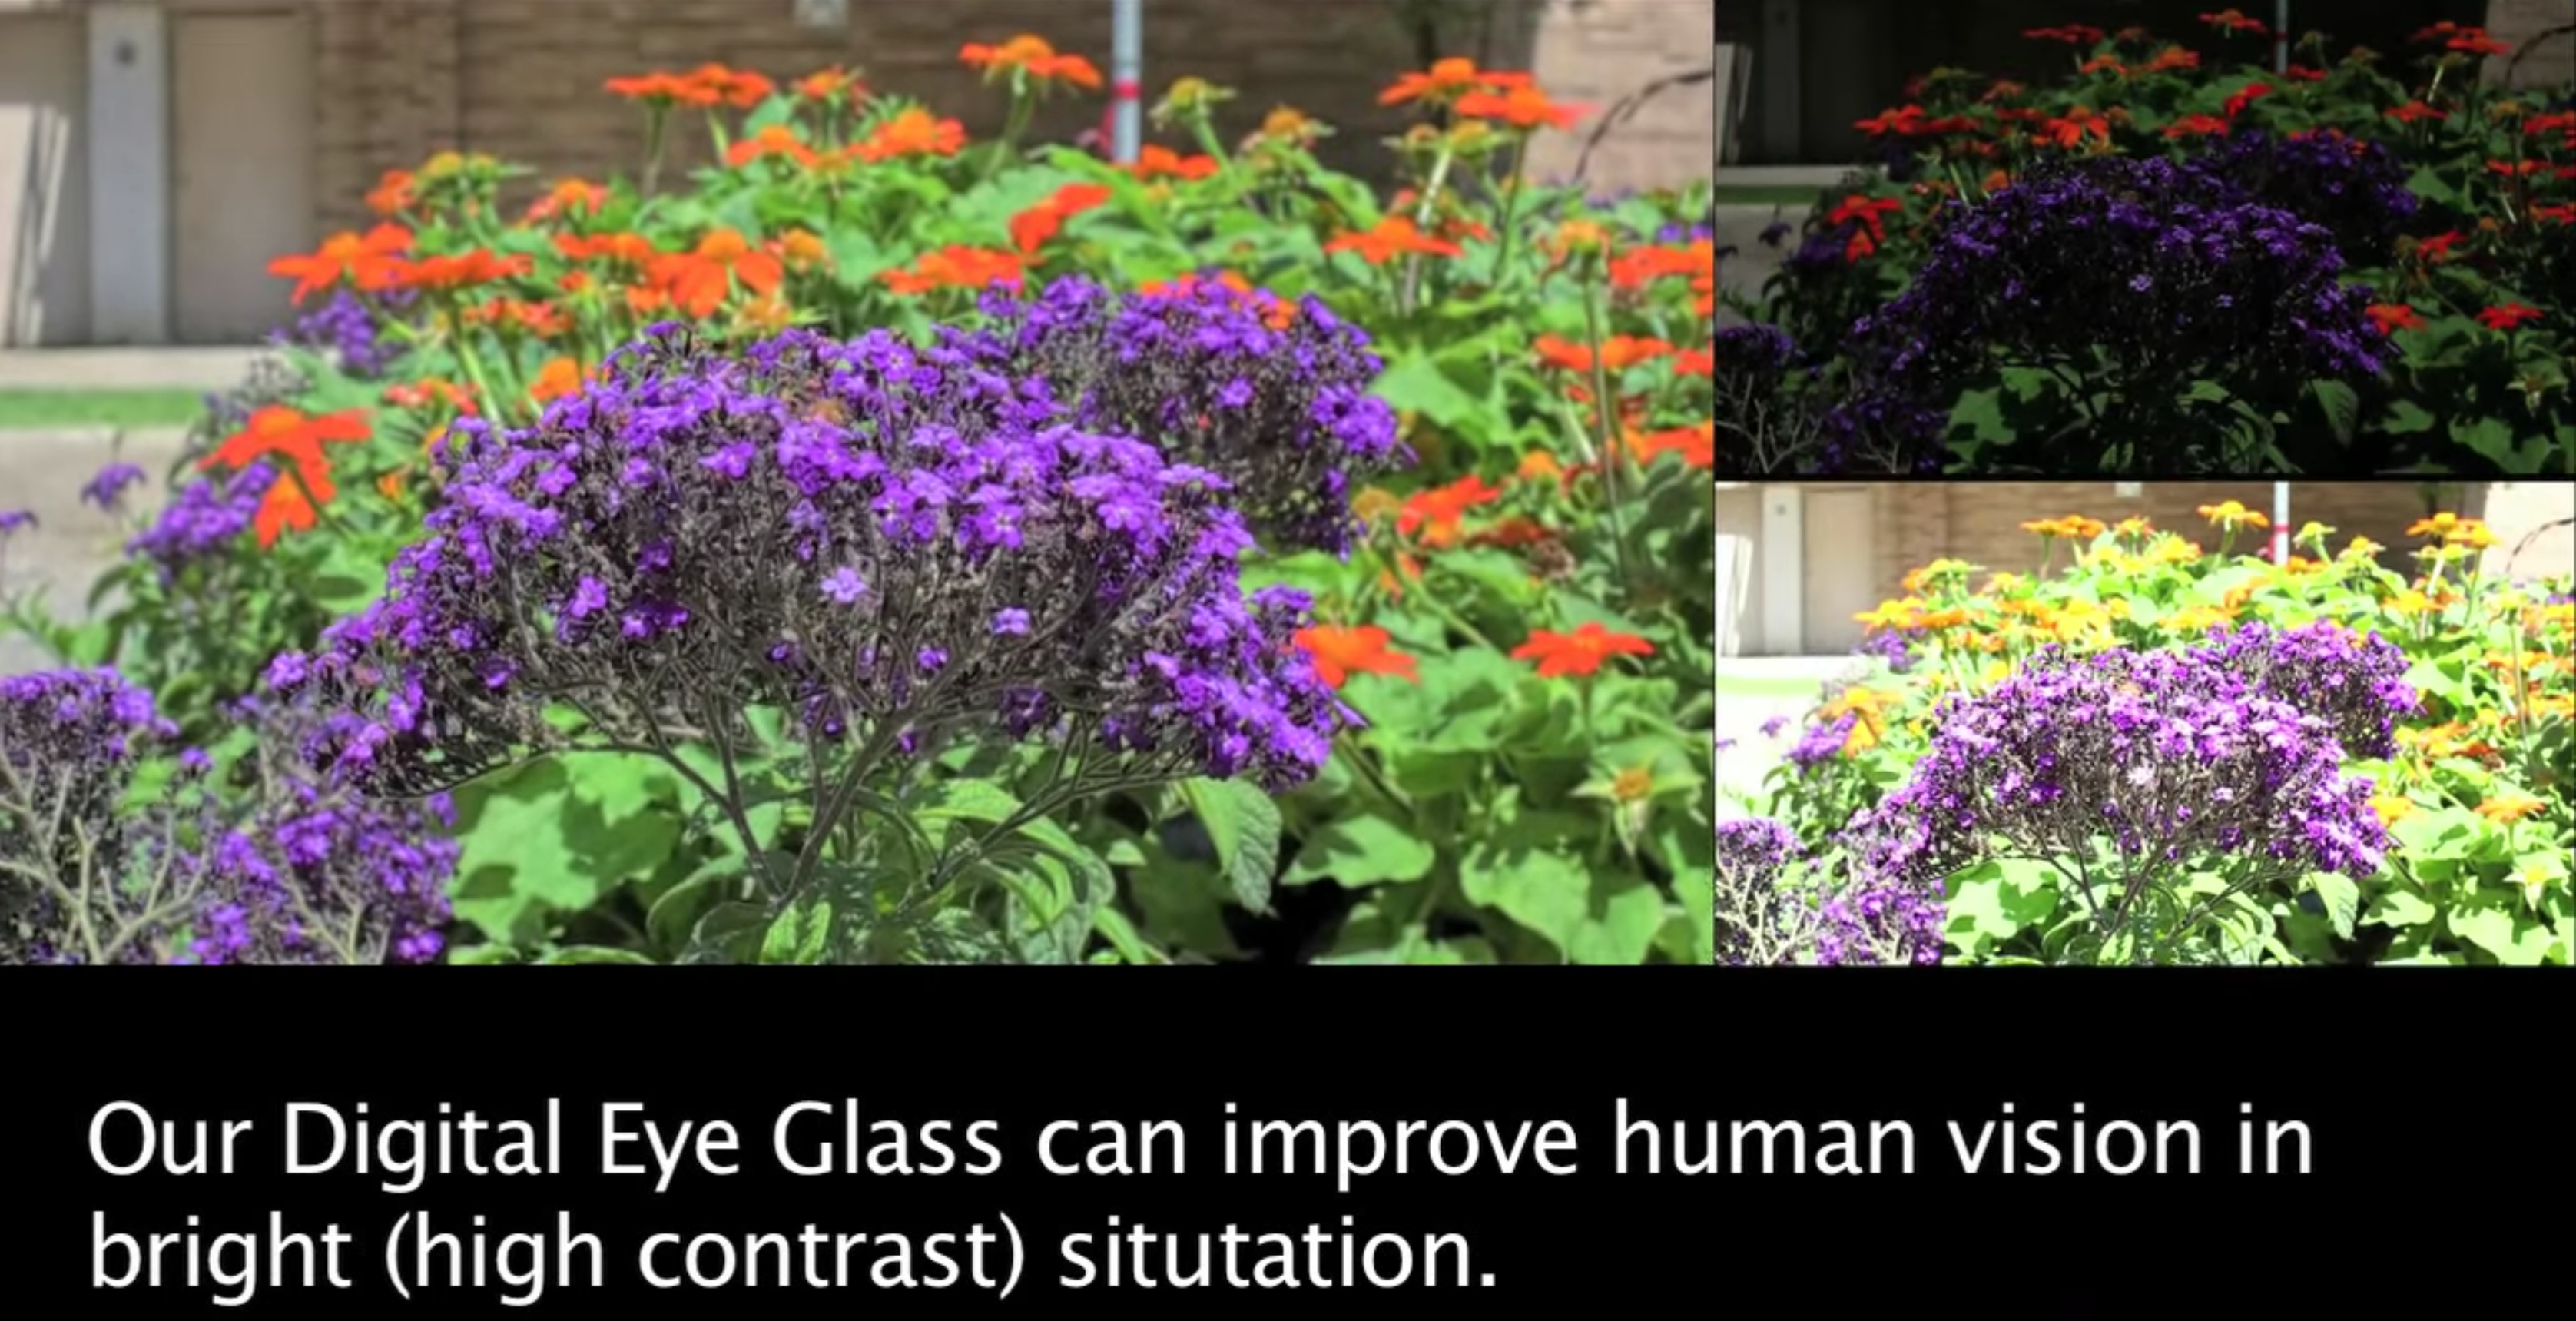
\includegraphics[width=5in]{ch2/diagrams/everyday1.png}
% \caption{}
% \label{fig:extremeeveryday1}
%\end{figure}
%
%\begin{figure}
%\center
% 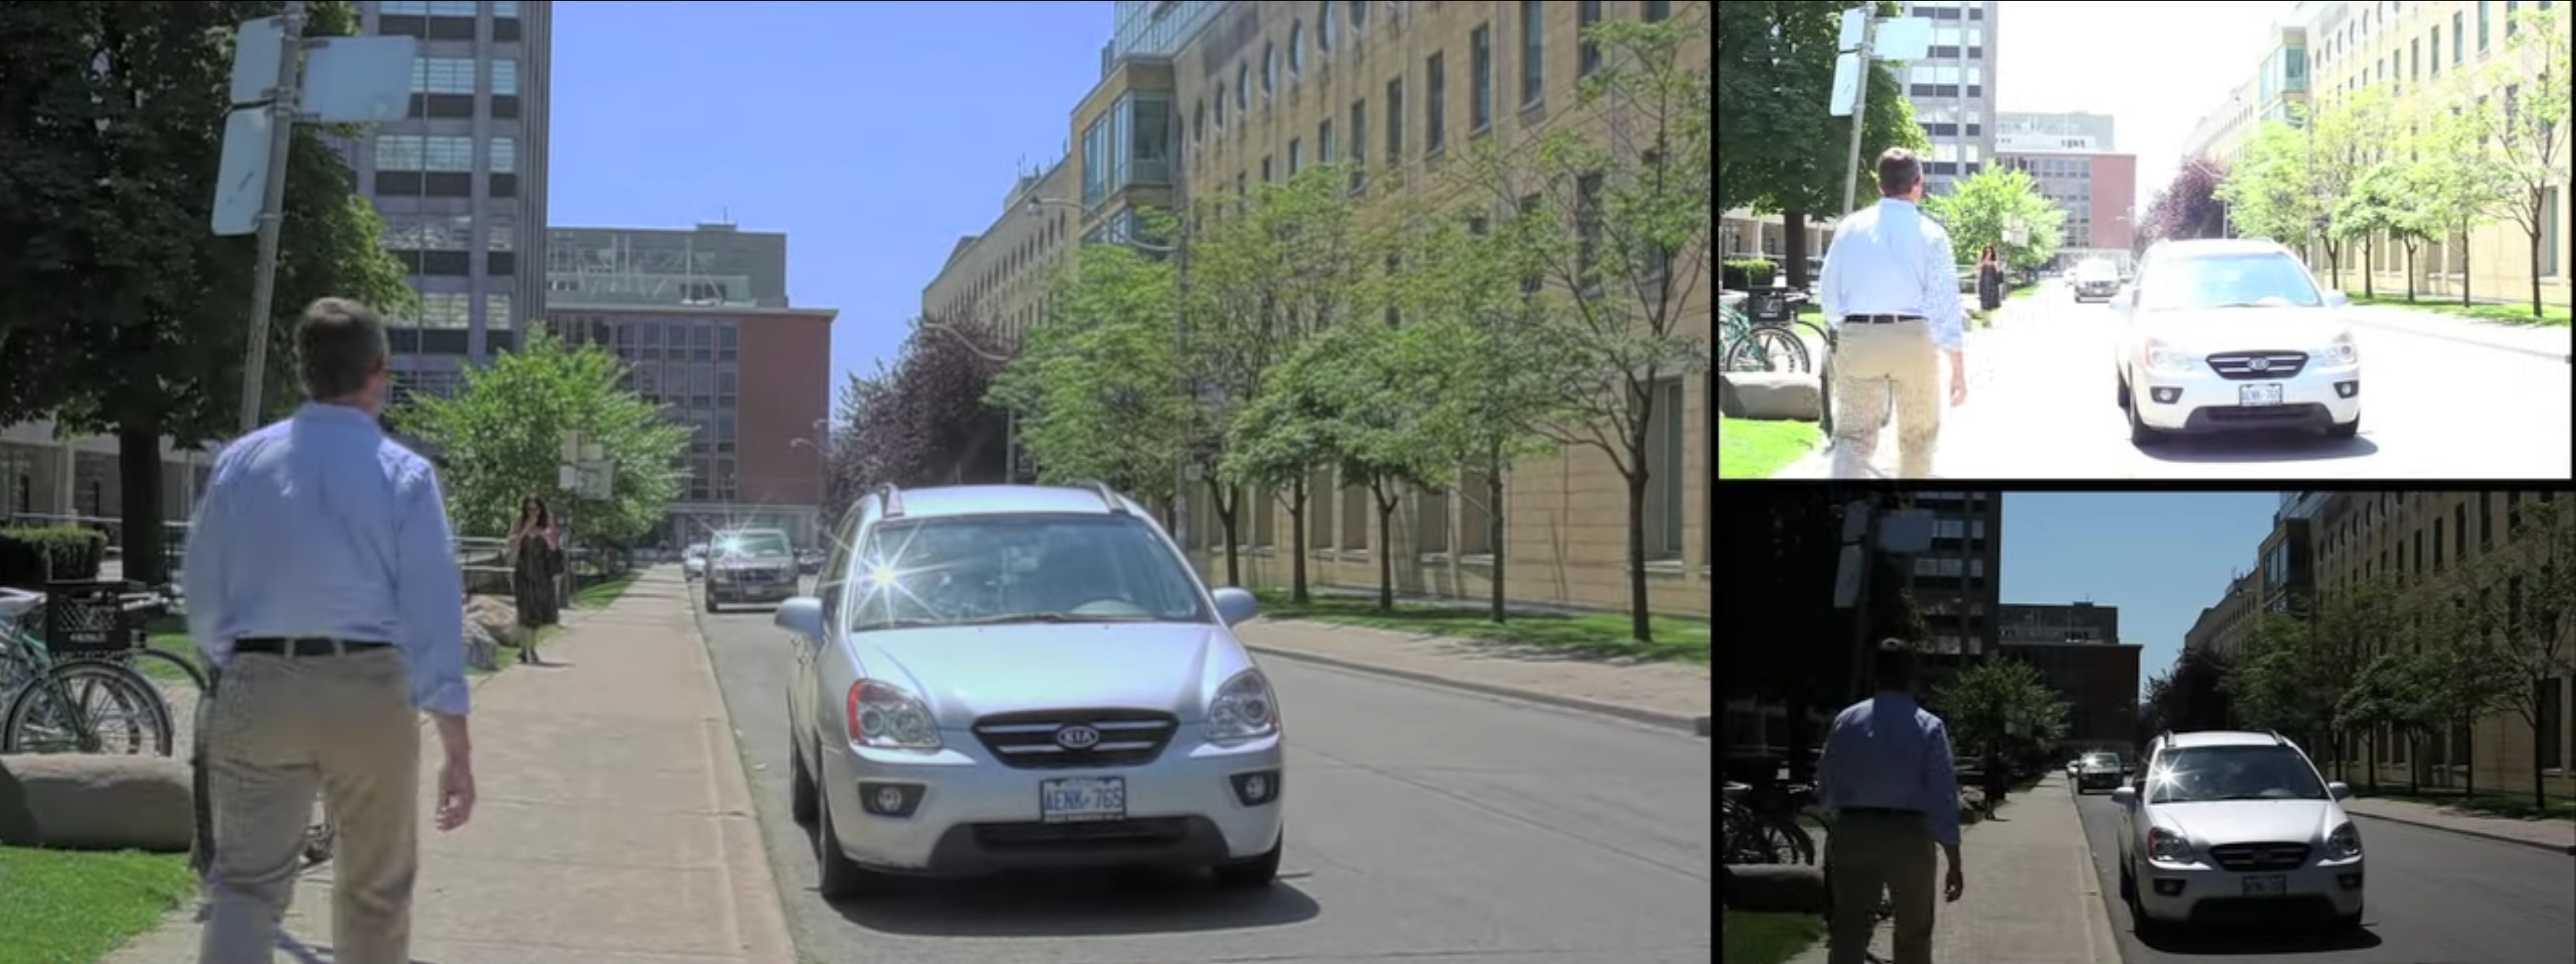
\includegraphics[width=5in]{ch2/diagrams/everyday2.png}
% \caption{}
% \label{fig:extremeeveryday2}
%\end{figure}
%
%\begin{figure}
%\center
% \includegraphics[width=5in]{ch2/diagrams/everyday3.png}
% \caption{}
% \label{fig:extremeeveryday3}
%\end{figure}
%
%\begin{figure}
%\center
% 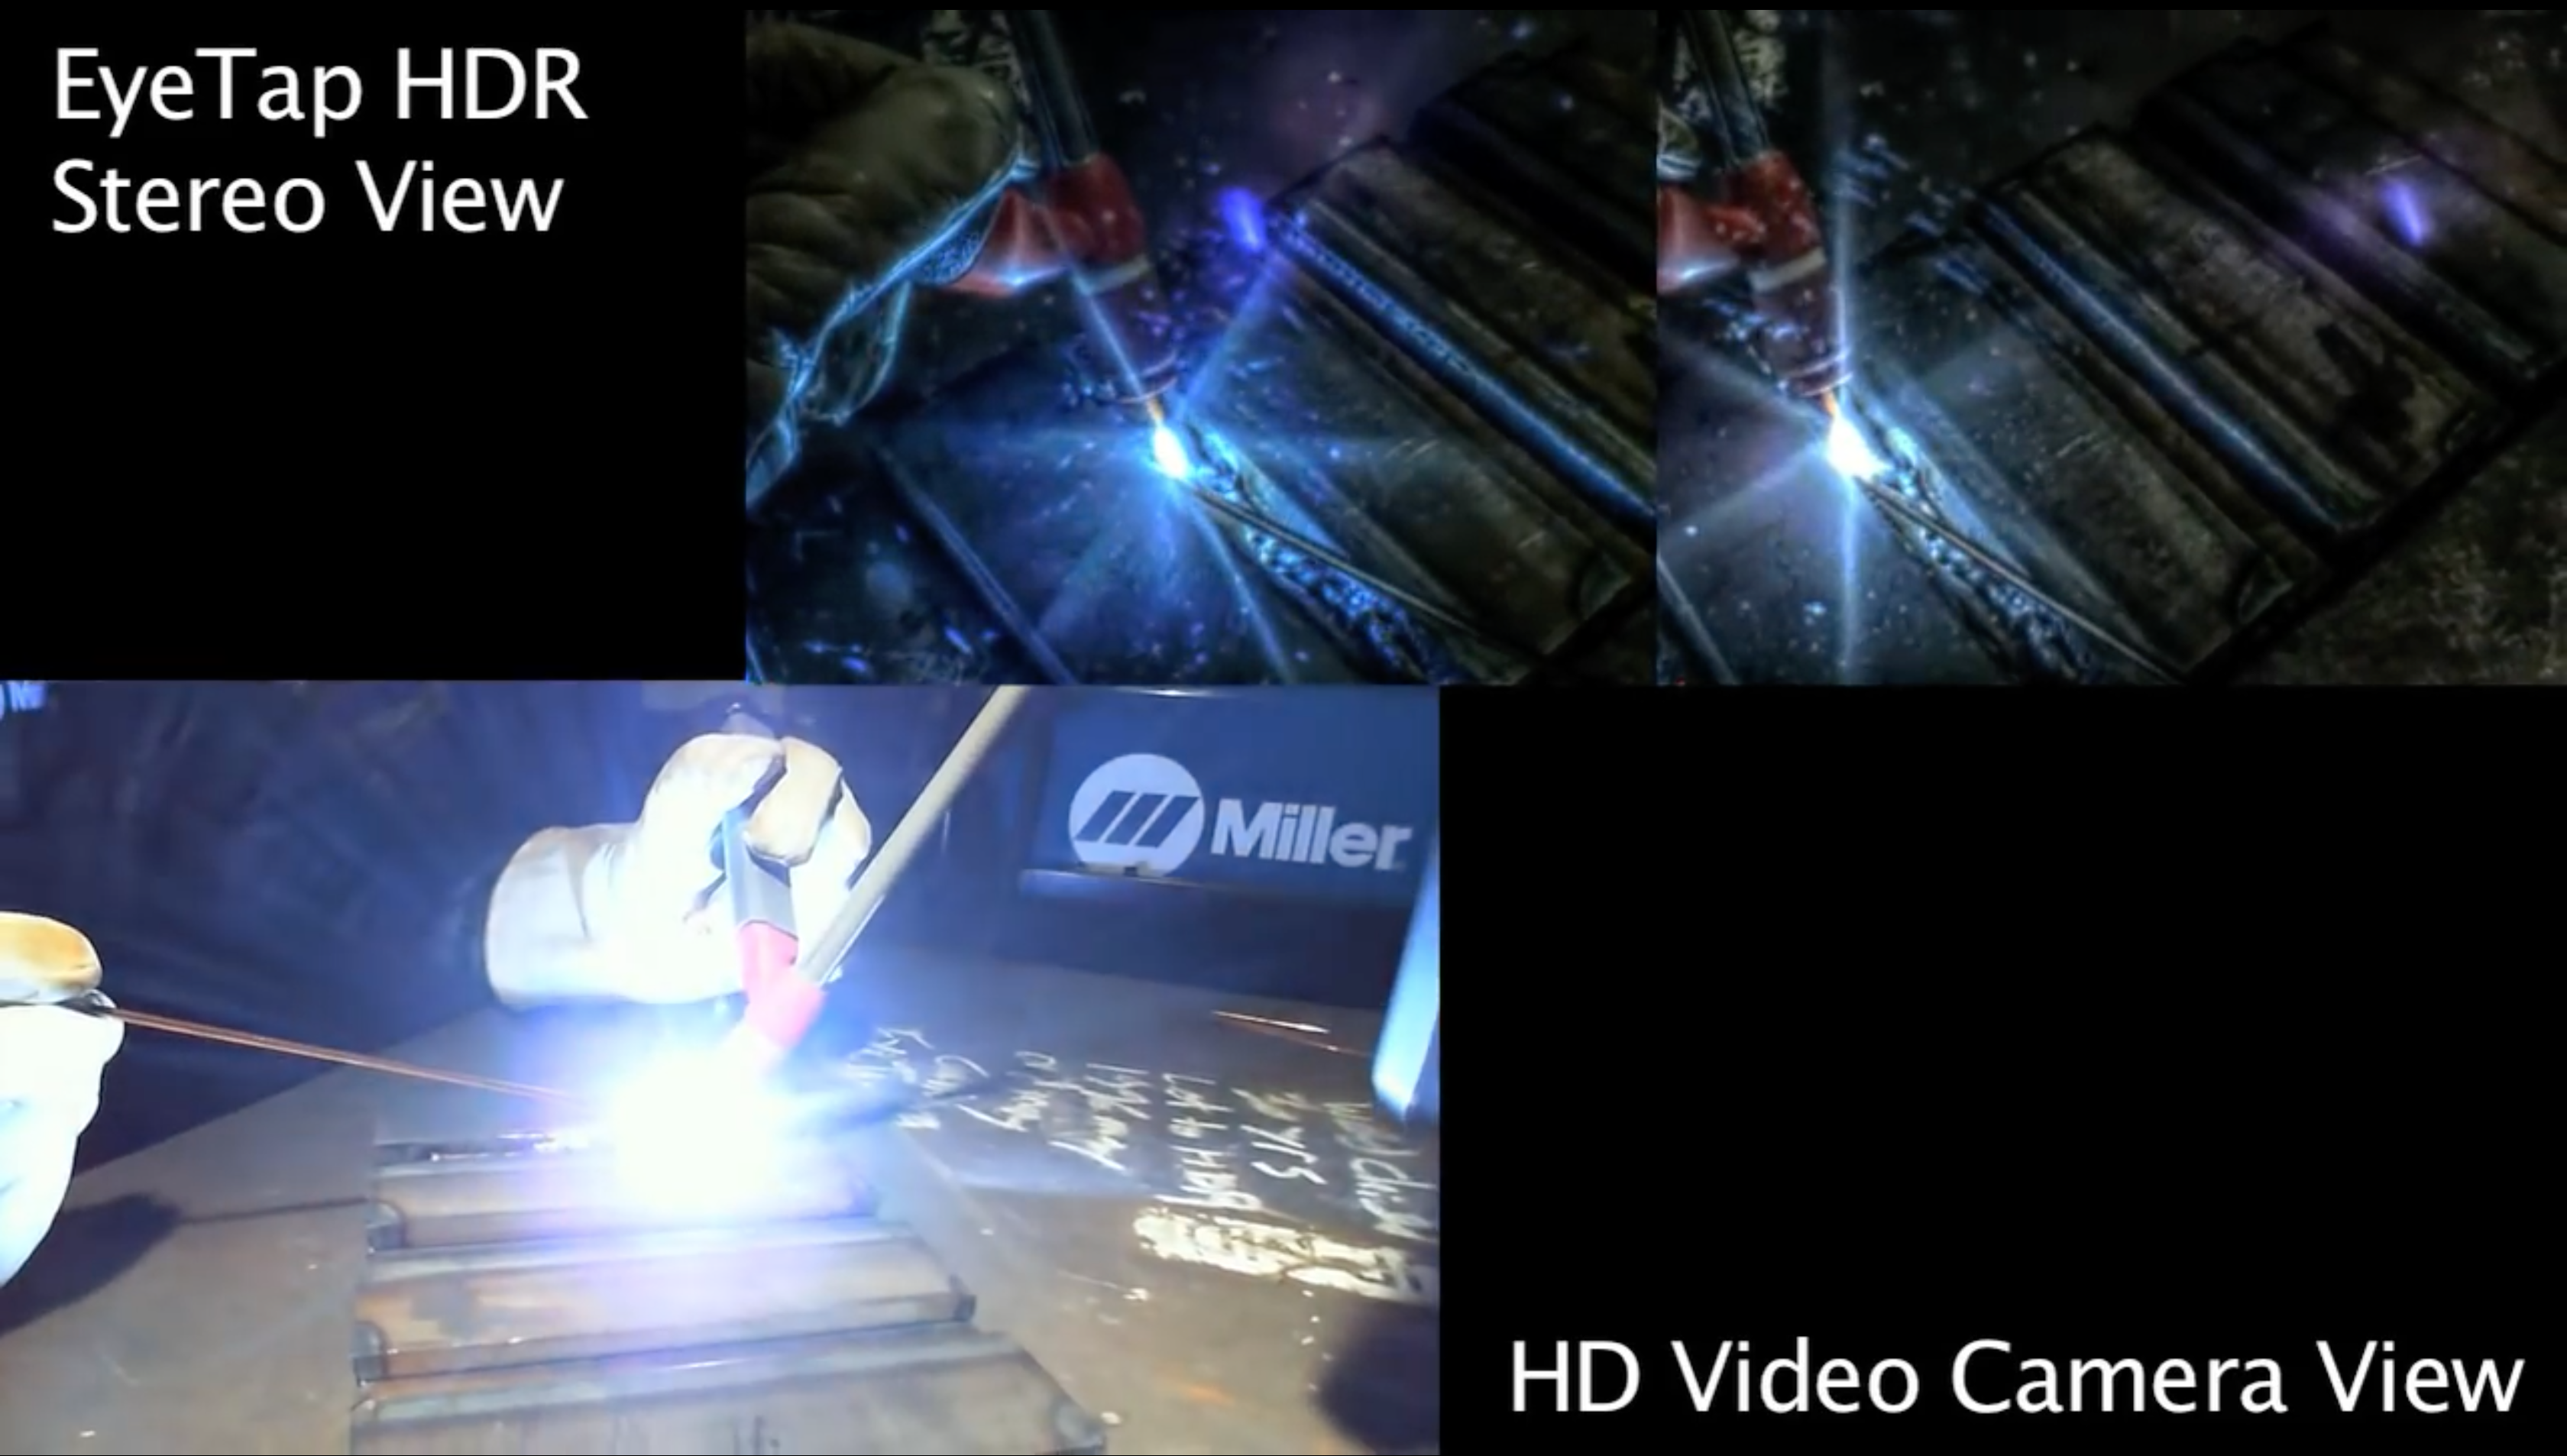
\includegraphics[width=5in]{ch2/diagrams/eyetap_3d_view.png}
% \caption{3D Stereoscopic View of the final HDR rendering. As we can see with ordinary HD video camera the bright light from the TID welding had completely `blinded' the sensor. }
% \label{fig:extreme3dhdr}
%\end{figure}
%
%
%\section{Conclusions and Discussion}
%We demonstrated the feasibility of using hardware to construct HDR video in realtime.  Our approach is parallelizable, and suitable for implementation on GPUs or FPGAs. To test our system, we have applied to TIG welding where extreme dynamic range scene is presented and also worn our seeing devices in our daily life.
%
%Similar to other HDR system which uses alternating exposures, image misalignment between the adjacent frames would product unpleasant ghosting artifacts. Numerous solutions have been proposed to address the image alignments between the consecutive frames. However, these solutions are computationally intense and not yet suitable for real-time usages. Alternatively, we can address this issue by optics which allows us to capture at the same instance, and thus our work in HDR video would be fully benefited from such hardware. 
%
